\documentclass[11pt, oneside]{article}
\usepackage{geometry}                		
\usepackage[utf8]{inputenc} 
\usepackage[spanish]{babel}
\geometry{letterpaper}                
\usepackage{graphicx}				
\usepackage{amssymb}
\usepackage{amsmath}
\usepackage{enumerate}
\usepackage{xcolor}
\usepackage{listings}

\lstset{basicstyle=\ttfamily,
  showstringspaces=false,
  commentstyle=\color{red},
  keywordstyle=\color{blue},
  aboveskip=3mm,
  belowskip=3mm,
  frame=tb
}

\title{Git y Github}

\begin{document}
\maketitle

\section{Introducción}
Git es un software de control de versiones ó CVS por sus siglas en Ingles. Este tipo de software están diseñados para porder llevar un contro de los cambios en un proyecto en el que esté involucrado el desarrollo de algun tipo de software.

Un ejemplo en el que git es usado bastante es cuando tenemos varias versiones de un proyecto:
\begin{itemize}
  \item tesis.docx
  \item tesis-terminada.docx
  \item tesis-terminada-final.docx
  \item tesis-terminada-fianl-definitiva.docx
\end{itemize}
En lugar de tener tantos archivos diferentes para llevar un control de los cambios, con git tendriamos un solo archivo y este mismo se encargaria de guardar registros de los cambios que se hagan en el proyecto. Aunque estos ejemplos son con archivos de word, git funciona mejor con archivos de texto por ejemplo; .txt, .csv, .c, .java, .tex, etc. Para git es mas dificil especificar los cambios para archivos empaquetados o binarios como .exe, .docx, .pptx, .jpeg, etc.

Otra gran ventaja de git es que permite a muchas personas colaborar en un solo proyecto, de esta forma se puede agilizar el proceso de desarrollo. Para colaborar se pueden utilizar herramientas que implementan el sistema de git como GitHub, GitLab, Bitbucket, etc.

\section{Instalar Git}
Para poder empezar a usar git tenemos que instalarlo, algunos sistemas como Mac o Linux lo podrían tener ya instalado, Windows no trae git instalado así que siempre es necesario instalarlo. Para revisar si ya estan instalados en estos sistemas es necesario abrir el terminal. En linux el terminal se abre presionando las teclas ctrl+alt+t y en Mac se puede abrir el terminal presionando las teclas cmd+espacio y luego ecribiendo la palabra terminal. Una vez abierto el terminal tenemos que escribir el commando:
\begin{lstlisting}[language=bash,caption={Comando para revisar versión de Git}]
git --version
\end{lstlisting}
Si lo tenemos instalado deberiamos ver una linea parecida a la siguiente:
\begin{lstlisting}[language=bash,caption={Versión de Git}]
git version 2.24.3 
\end{lstlisting}
Si no lo tenemos instalado veremos algo parecido a esto:
\begin{lstlisting}[language=bash,caption={Git no instalado}]
Unknown command: git
\end{lstlisting}

En caso que git no este instalado tendremos que ir al sito web \url{https://git-scm.com/downloads} y darle click al botón de descargar. En la figura \ref{fig:git} se muestra la pagina donde descargar git.
\begin{figure}[h]
  \centering
  \caption{Sitio web de git}
  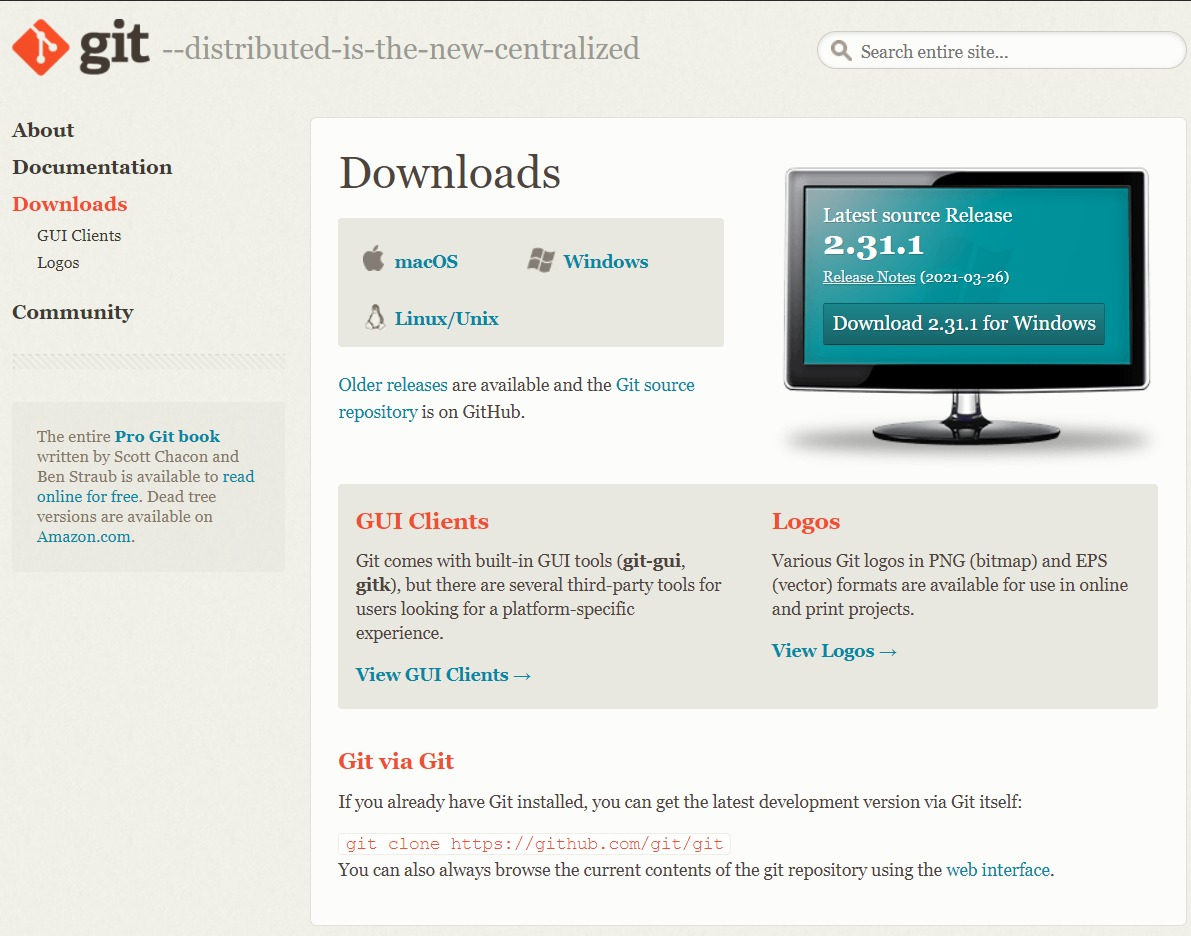
\includegraphics[width=0.70\textwidth]{./img/ind-from-web.jpeg}
  \label{fig:git-web}
\end{figure}

\subsection{Windows}
\subsection{Mac}
\subsection{Linux}

\section{GitHub}

\section{Integración con VSCode}
\section{Integración con VSCode}

\end{document}
